% Provenance (never printed): see sources/outline_sources.md (Year 1:
% geological cross-sections, apparent dip, thickness, boreholes). Every
% Varden Hills number comes from figdata/bachelor-1/varden_sections.py, which
% imports the shared model figdata/shared/region.py; numbers of the exercises
% and problem in the Book 3 scratch calculator and in that script's values.
\chapter{Cross-Sections}\label{ch:b1:cross-sections}

An engineering company plans a tunnel under the Varden Hills, straight from
west to east at a constant elevation of \qty{200}{m}. Before a single metre
is bored, the geologists must say which rocks the machine will cut, where it
will cross the fault, and how long it will spend in the limestone, a rock
that may hold open cavities and water. Nobody can see inside the hills; but
the \omterm{def:b1:geological-maps:geological-map}{geological map} of \cref{ch:b1:geological-maps}, a few boreholes and the
geometry of planes are enough to draw a vertical slice through the ground ---
a cross-section --- and to read the answers from it. This chapter teaches how
a section is built from a map, how \omterm{def:b1:geological-maps:attitude}{dips} and thicknesses change when a slice
is cut obliquely, how boreholes are correlated, and how a section tells the
history of the rocks it cuts. It ends with the tunnel.

\begin{recall}
The \omterm{def:b1:geological-maps:attitude}{attitude} of a plane is given by its \omterm{def:b1:geological-maps:attitude}{dip direction} $\alpha$ and its \omterm{def:b1:geological-maps:attitude}{dip}
$\delta$, and the plane through a point of elevation $z_0$ at the origin is
$z = z_0 - \tan\delta\,(x\sin\alpha + y\cos\alpha)$; three points of a
contact fix its \omterm{def:b1:geological-maps:attitude}{attitude}; the V-rule reads the \omterm{def:b1:geological-maps:attitude}{dip} from the \omterm{def:b1:geological-maps:geological-map}{outcrop} pattern
in valleys (\cref{ch:b1:geological-maps}). A contour line joins points of
equal elevation on a topographic map (Book 1, grade 9). Younger rocks lie on
older ones, and whatever cuts a rock is younger than it (Book 1, grade 7).
\end{recall}

\section{From the map to the section}

\begin{definition}[Geological cross-section, topographic profile, vertical exaggeration]\label{def:b1:cross-sections:section}
A \emph{geological cross-section}\index{geological cross-section} is a
drawing of the rock units and structures in a vertical plane through the
ground, along a line drawn on the map. Its upper edge is the
\emph{topographic profile}\index{topographic profile}, the curve of ground
elevation along the line. The \emph{vertical
exaggeration}\index{vertical exaggeration} $e$ of a section is the ratio of
its vertical scale to its horizontal scale; a section is \emph{true to
scale} when $e = 1$.
\end{definition}

\begin{method}[Constructing a cross-section from a map]\label{met:b1:cross-sections:construct}
\begin{enumerate}
  \item Draw the line of section on the map and lay the edge of a strip of
        paper along it; mark where each contour line crosses it, with its
        elevation, and where each contact and fault crosses it.
  \item Draw a horizontal base line of the same length and a vertical scale
        of elevation (choose $e$, and write it on the section).
  \item Transfer each contour mark to its elevation and join the points
        smoothly: this is the \omterm{def:b1:cross-sections:section}{topographic profile}.
  \item Transfer each contact and fault to the profile, at the point where it
        crosses the line.
  \item From each such point, draw the contact into the ground with its
        \omterm{def:b1:geological-maps:attitude}{dip} \emph{in the plane of the section} --- its \omterm{def:b1:cross-sections:apparent-dip}{apparent dip}
        (\cref{sec:b1:cross-sections:apparent}) --- exaggerated by $e$ if
        $e \ne 1$; use boreholes and \omterm{def:b1:cross-sections:structure-contour}{structure contours} where there are any.
  \item Complete the units between the \omterm{def:b1:geological-maps:geological-map}{contacts}, respecting the order of
        superposition and the cuts, and add the legend, the scales, the
        orientation of the line and $e$.
\end{enumerate}
\end{method}

\begin{omfigure}
\begin{tikzpicture}[font=\scriptsize, x=1cm, y=1cm]
% map strip with contours crossing the section line
\draw[black!50] (0,2.7) rectangle (9,4.5);
\foreach \x/\h in {0.7/300, 1.6/350, 2.6/400, 4.1/400, 5.0/350, 5.8/300, 7.2/300, 8.2/350} {
  \draw[contour, brown!70!black] (\x-0.25,2.7) .. controls (\x+0.1,3.4) and (\x-0.1,3.8) .. (\x+0.2,4.5);
  \node[brown!60!black, above] at (\x+0.2,4.5) {\h};
}
\draw[omThm, thick] (0,3.6) node[left] {X} -- (9,3.6) node[right] {Y};
\fill[omDef] (3.4,3.6) circle (1.5pt);
\node[omDef, fill=white, inner sep=1pt, above right] at (3.4,3.62) {contact};
% profile
\draw[->] (0,-0.1) -- (0,1.95) node[above] {elevation (m)};
\draw (0,0) -- (9,0);
\foreach \y/\l in {0/250, 0.5/300, 1.0/350, 1.5/400} { \draw (-0.08,\y) -- (0,\y); \node[left] at (-0.08,\y) {\l}; }
\coordinate (p1) at (0.85,0.5); \coordinate (p2) at (1.75,1.0); \coordinate (p3) at (2.75,1.5);
\coordinate (p4) at (4.25,1.5); \coordinate (p5) at (5.15,1.0); \coordinate (p6) at (5.95,0.5);
\coordinate (p7) at (7.35,0.5); \coordinate (p8) at (8.35,1.0);
\foreach \i/\x in {1/0.85,2/1.75,3/2.75,4/4.25,5/5.15,6/5.95,7/7.35,8/8.35} {
  \draw[black!35, densely dotted] (\x,3.6) -- (p\i);
  \fill (p\i) circle (1.2pt);
}
\draw[thick] (0,0.2) .. controls (0.5,0.3) .. (p1) .. controls (1.3,0.8) .. (p2) .. controls (2.3,1.35) .. (p3)
  .. controls (3.5,1.85) .. (p4) .. controls (4.7,1.25) .. (p5) .. controls (5.5,0.7) .. (p6)
  .. controls (6.6,0.25) .. (p7) .. controls (7.9,0.75) .. (p8) .. controls (8.7,1.15) .. (9,1.2);
\draw[omDef, densely dotted] (3.4,3.6) -- (3.4,1.72);
\draw[omDef, thick] (3.4,1.72) -- (4.45,0.05);
\node[omDef, below right] at (4.3,-0.02) {contact, drawn with its apparent dip};
\end{tikzpicture}

{\small Building a section (schematic): the crossings of the contour lines
with the line X--Y are carried down to their elevations to give the
\omterm{def:b1:cross-sections:section}{topographic profile}; a contact crossing the line is carried down to the
profile and drawn into the ground with its \omterm{def:b1:cross-sections:apparent-dip}{apparent dip}.}
\end{omfigure}

The section below was built by computer from the model of the Varden Hills
along the line C--D, which runs due east across the map at $y = \qty{6}{km}$.
It shows the \omterm{def:b1:geological-maps:fold}{anticline} whose core of sandstone and basement appears at
$x \approx \qty{3.5}{km}$, the limestone and shale on its limbs, the chalk in
the \omterm{def:b1:geological-maps:fold}{syncline} to the east, and the normal fault. The tunnel line, at
\qty{200}{m}, and the boreholes B1, B2, B3 of
\cref{sec:b1:cross-sections:boreholes} are drawn on it.

\begin{omfigure}
\begin{tikzpicture}
\begin{axis}[x=1.4cm, y=0.0042cm, xmin=0, xmax=10, ymin=-500, ymax=650,
  axis on top, tick label style={font=\scriptsize}, label style={font=\small},
  xlabel={distance east from C (km)}, ylabel={elevation (m)},
  ytick={-400,-200,0,200,400,600}, clip=true]
\addplot[lith schist, draw=black, line width=0.3pt, even odd rule] table {figdata/out/bachelor-1-varden_sections-cd-unit-schist.dat};
\addplot[lith granite, draw=black, line width=0.3pt, even odd rule] table {figdata/out/bachelor-1-varden_sections-cd-unit-granite.dat};
\addplot[om lith={icsTriassic!35}{om sand}, draw=black, line width=0.3pt, even odd rule] table {figdata/out/bachelor-1-varden_sections-cd-unit-sandstone.dat};
\addplot[om lith={icsJurassic!40}{om limestone}, draw=black, line width=0.3pt, even odd rule] table {figdata/out/bachelor-1-varden_sections-cd-unit-limestone.dat};
\addplot[om lith={icsJurassic!15}{om shale}, draw=black, line width=0.3pt, even odd rule] table {figdata/out/bachelor-1-varden_sections-cd-unit-shale.dat};
\addplot[om lith={icsCretaceous!35}{om limestone}, draw=black, line width=0.3pt, even odd rule] table {figdata/out/bachelor-1-varden_sections-cd-unit-chalk.dat};
\addplot[lith alluvium, draw=black, line width=0.3pt, even odd rule] table {figdata/out/bachelor-1-varden_sections-cd-unit-alluvium.dat};
\addplot[black, line width=0.8pt] table {figdata/out/bachelor-1-varden_sections-cd-ground.dat};
\addplot[fault, line width=1.1pt] table {figdata/out/bachelor-1-varden_sections-cd-fault.dat};
\addplot[omThm, line width=1.4pt] coordinates {(1,200) (9,200)};
\node[omThm, font=\scriptsize, fill=white, inner sep=1pt, below] at (axis cs:8.3,190) {tunnel, \qty{200}{m}};
\draw[blue!60!black, line width=0.9pt] (axis cs:1.5,-480) -- (axis cs:1.5,524);
\draw[blue!60!black, line width=0.9pt] (axis cs:3.5,-480) -- (axis cs:3.5,381);
\draw[blue!60!black, line width=0.9pt] (axis cs:5.5,-480) -- (axis cs:5.5,530);
\node[font=\scriptsize, blue!60!black, fill=white, inner sep=1pt] at (axis cs:1.5,-440) {B1};
\node[font=\scriptsize, blue!60!black, fill=white, inner sep=1pt] at (axis cs:3.5,-440) {B2};
\node[font=\scriptsize, blue!60!black, fill=white, inner sep=1pt] at (axis cs:5.5,-440) {B3};
\node[font=\small, above right] at (axis cs:0,650) {C (west)};
\node[font=\small, above left] at (axis cs:10,650) {D (east)};
\end{axis}
\end{tikzpicture}

\smallskip
\begin{tikzpicture}
\begin{axis}[x=1.4cm, y=0.0014cm, xmin=0, xmax=10, ymin=-500, ymax=650,
  axis on top, tick label style={font=\scriptsize}, ytick={-500,0,500},
  xticklabels={}, clip=true]
\addplot[lith schist, draw=black, line width=0.2pt, even odd rule] table {figdata/out/bachelor-1-varden_sections-cd-unit-schist.dat};
\addplot[lith granite, draw=black, line width=0.2pt, even odd rule] table {figdata/out/bachelor-1-varden_sections-cd-unit-granite.dat};
\addplot[om lith={icsTriassic!35}{om sand}, draw=black, line width=0.2pt, even odd rule] table {figdata/out/bachelor-1-varden_sections-cd-unit-sandstone.dat};
\addplot[om lith={icsJurassic!40}{om limestone}, draw=black, line width=0.2pt, even odd rule] table {figdata/out/bachelor-1-varden_sections-cd-unit-limestone.dat};
\addplot[om lith={icsJurassic!15}{om shale}, draw=black, line width=0.2pt, even odd rule] table {figdata/out/bachelor-1-varden_sections-cd-unit-shale.dat};
\addplot[om lith={icsCretaceous!35}{om limestone}, draw=black, line width=0.2pt, even odd rule] table {figdata/out/bachelor-1-varden_sections-cd-unit-chalk.dat};
\addplot[lith alluvium, draw=black, line width=0.2pt, even odd rule] table {figdata/out/bachelor-1-varden_sections-cd-unit-alluvium.dat};
\addplot[black, line width=0.6pt] table {figdata/out/bachelor-1-varden_sections-cd-ground.dat};
\addplot[fault, line width=0.8pt] table {figdata/out/bachelor-1-varden_sections-cd-fault.dat};
\end{axis}
\end{tikzpicture}

{\small Section C--D across the Varden Hills, from the model of the region.
Top: \omterm{def:b1:cross-sections:section}{vertical exaggeration} $e = 3$; bottom: the same section true to scale
($e = 1$), where the \ang{12} limbs look as gentle as they are. Colours as in
the \omterm{def:b1:geological-maps:geological-map}{geological map} of \cref{ch:b1:geological-maps}; the fault (thick line)
is the normal fault, its eastern block downthrown. The red line is the
tunnel of the problem; B1--B3 are boreholes.}
\end{omfigure}

\omterm{def:b1:cross-sections:section}{Vertical exaggeration} makes thin units and gentle relief readable, but it
distorts every angle: the \ang{12} limbs of the \omterm{def:b1:geological-maps:fold}{fold} appear at about
\ang{32} in the upper section. The next section says exactly how.

\section{Apparent dip}\label{sec:b1:cross-sections:apparent}

\begin{definition}[Apparent dip]\label{def:b1:cross-sections:apparent-dip}
The \emph{apparent dip}\index{apparent dip} $\beta$ of a plane in a given
vertical section is the angle between the horizontal and the trace of the
plane in that section. It equals the true \omterm{def:b1:geological-maps:attitude}{dip} $\delta$ when the section runs
along the \omterm{def:b1:geological-maps:attitude}{dip direction}, and is zero when it runs along the \omterm{def:b1:geological-maps:attitude}{strike}.
\end{definition}

\begin{theorem}[Apparent dip]\label{thm:b1:cross-sections:apparent-dip}
A plane of \omterm{def:b1:geological-maps:attitude}{dip} $\delta$ and \omterm{def:b1:geological-maps:attitude}{dip direction} $\alpha$, cut by a vertical
section of \omterm{def:b1:spherical-astronomy:horizontal}{azimuth} $\theta$, shows the \omterm{def:b1:cross-sections:apparent-dip}{apparent dip} $\beta$ with
\[
  \tan\beta = \tan\delta\,\cos\gamma, \qquad \gamma = \alpha - \theta ,
\]
the plane going down in the direction $\theta$ when $\cos\gamma > 0$.
In particular $|\beta| \le \delta$, with equality only along the \omterm{def:b1:geological-maps:attitude}{dip
direction}.
\end{theorem}

\begin{proof}
Take the plane $z = z_0 - \tan\delta\,(x\sin\alpha + y\cos\alpha)$ of
\cref{ch:b1:geological-maps}. Along the section, a horizontal step of length
$s$ in the direction $\theta$ is $(x, y) = s(\sin\theta, \cos\theta)$, so
$z = z_0 - s\tan\delta\,(\sin\theta\sin\alpha + \cos\theta\cos\alpha) =
z_0 - s\tan\delta\cos(\alpha - \theta)$. The trace is a straight line that
descends by $\tan\delta\cos\gamma$ per unit horizontal distance: that is
$\tan\beta$. Since $|\cos\gamma| \le 1$, $|\tan\beta| \le \tan\delta$.
\end{proof}

\begin{omfigure}
\begin{tikzpicture}[font=\scriptsize, x={(1cm,0cm)}, y={(0.6cm,0.45cm)}, z={(0cm,1cm)}]
% hidden edges of the block
\draw[black!30, densely dashed] (0,0,0) -- (0,3,0) -- (4,3,0);
\draw[black!30, densely dashed] (0,3,0) -- (0,3,2);
% the oblique vertical section, from the front-left corner to the back-right one
\fill[black!10, opacity=0.7] (0,0,0) -- (4,3,0) -- (4,3,2) -- (0,0,2) -- cycle;
\draw[black!45] (0,0,0) -- (4,3,0) -- (4,3,2);
% the dipping plane, from the top-west edge down to the base
\fill[omDef!25, opacity=0.75] (0,0,2) -- (2.6,0,0) -- (2.6,3,0) -- (0,3,2) -- cycle;
\draw[omDef] (2.6,0,0) -- (2.6,3,0);
\draw[omDef, very thick] (0,0,2) -- (2.6,0,0);
\draw[omThm, very thick] (0,0,2) -- (2.6,1.95,0);
% visible edges of the block
\draw[black!70] (0,0,0) -- (4,0,0) -- (4,0,2) -- (0,0,2) -- cycle;
\draw[black!70] (0,0,2) -- (0,3,2) -- (4,3,2) -- (4,0,2);
\draw[black!70] (4,0,0) -- (4,3,0) -- (4,3,2);
% labels
\draw[omDef] (2.0,0,0) arc[start angle=180, end angle=142.4, radius=0.6cm];
\node[omDef] at (1.7,0,0.2) {$\delta$};
\node[omDef, below, align=center] at (1.3,0,0) {front face, along the dip direction:\\ true dip $\delta$};
\node[omThm, right, align=left] at (4.45,2.2,0.3) {oblique section (grey):\\ apparent dip $\beta < \delta$};
\node[above] at (0,1.5,2) {N};
\draw[->] (0.15,1.5,2.05) -- (0.15,2.2,2.05);
\end{tikzpicture}

{\small \omterm{def:b1:cross-sections:apparent-dip}{Apparent dip} (schematic block). A plane dipping east (blue) shows its
true \omterm{def:b1:geological-maps:attitude}{dip} $\delta$ on the front face, a vertical face cut along the \omterm{def:b1:geological-maps:attitude}{dip
direction}; on the grey vertical section, cut obliquely, its trace (red)
descends more gently, with the \omterm{def:b1:cross-sections:apparent-dip}{apparent dip} $\beta$; on a section along the
\omterm{def:b1:geological-maps:attitude}{strike}, north--south, it would be horizontal.}
\end{omfigure}

\begin{proposition}[Angles in an exaggerated section]\label{prop:b1:cross-sections:exaggeration}
In a section drawn with \omterm{def:b1:cross-sections:section}{vertical exaggeration} $e$, a line of \omterm{def:b1:cross-sections:apparent-dip}{apparent dip}
$\beta$ is drawn at the angle $\beta'$ with $\tan\beta' = e\tan\beta$.
\end{proposition}

\begin{proof}
Over a horizontal distance $s$ the line drops by $s\tan\beta$; drawn with
vertical scale $e$ times the horizontal scale, the drop appears as
$es\tan\beta$ over the same drawn length $s$.
\end{proof}

\begin{example}
The east limb of the Varden \omterm{def:b1:geological-maps:fold}{anticline} \omterm{def:b1:geological-maps:attitude}{dips} \ang{12.16} toward \ang{080.7}
(\cref{ch:b1:geological-maps}). In the east--west section C--D,
$\gamma = \ang{80.7} - \ang{90} = \ang{-9.3}$, and $\tan\beta =
\tan\ang{12.16}\cos\ang{9.3} = 0.2154\times0.9868 = 0.2126$: $\beta =
\ang{12.0}$. Drawn with $e = 3$, it appears at $\arctan(3\times0.2126) =
\ang{32.5}$. In the section A--B of \omterm{def:b1:spherical-astronomy:horizontal}{azimuth} \ang{071.6}, $\gamma = \ang{9.1}$
and $\beta = \ang{12.0}$ as well: both sections run close to the \omterm{def:b1:geological-maps:attitude}{dip
direction}. The fault, which \omterm{def:b1:geological-maps:attitude}{dips} \ang{60} toward \ang{120}, has in C--D the
\omterm{def:b1:cross-sections:apparent-dip}{apparent dip} $\arctan(\tan\ang{60}\cos\ang{30}) = \arctan 1.5 = \ang{56.3}$.
\end{example}

\section{Thickness}

\begin{definition}[True thickness, vertical thickness]\label{def:b1:cross-sections:thickness}
The \emph{true thickness}\index{true thickness} $t$ of a layer is the
distance between its base and its top measured perpendicular to the
bedding. Its \emph{vertical thickness}\index{vertical thickness} $h$ is the
same distance measured along the vertical, as a vertical borehole meets it.
\end{definition}

\begin{proposition}[Thickness of a dipping layer]\label{prop:b1:cross-sections:thickness}
For a layer of \omterm{def:b1:geological-maps:attitude}{dip} $\delta$:
\begin{enumerate}
  \item $t = h\cos\delta$;
  \item on horizontal ground, if the \omterm{def:b1:geological-maps:geological-map}{outcrop} of the layer has the width $w$
        measured perpendicular to the \omterm{def:b1:geological-maps:attitude}{strike}, $t = w\sin\delta$;
  \item on ground sloping at the angle $\sigma$ in the direction
        perpendicular to the \omterm{def:b1:geological-maps:attitude}{strike}, with $w$ measured along the ground,
        $t = w\sin(\delta + \sigma)$ if the ground slopes the opposite way to
        the \omterm{def:b1:geological-maps:attitude}{dip}, and $t = w\sin(\delta - \sigma)$ if it slopes the same way
        less steeply than the beds.
\end{enumerate}
\end{proposition}

\begin{proof}
In the vertical plane perpendicular to the \omterm{def:b1:geological-maps:attitude}{strike}, the base and the top of
the layer are two parallel lines inclined at $\delta$, a distance $t$ apart.
(1) A vertical segment joining them makes the angle $\delta$ with their
common normal, so $t = h\cos\delta$. (2)--(3) A segment of length $w$ joining
them along the ground makes with the bedding the angle $\delta$ when the
ground is flat, $\delta + \sigma$ when the ground rises toward the \omterm{def:b1:geological-maps:attitude}{dip
direction}'s opposite (the two inclinations add), and $\delta - \sigma$ when
it falls the same way; the distance between the parallel lines is the
length of the segment times the sine of that angle.
\end{proof}

\begin{omfigure}
\begin{tikzpicture}[font=\scriptsize]
\pgfmathsetmacro{\d}{25}\pgfmathsetmacro{\t}{1.3}
\pgfmathsetmacro{\h}{\t/cos(\d)}\pgfmathsetmacro{\w}{\t/sin(\d)}
\pgfmathsetmacro{\X}{4.0}
\fill[icsJurassic!30] (-\w,0) -- (0,0) -- (\X,{-\X*tan(\d)}) -- (\X,{-\X*tan(\d)-\h}) -- cycle;
\draw[thick] (0,0) -- (\X,{-\X*tan(\d)}) node[right] {top of the layer};
\draw[thick] (-\w,0) -- (\X,{-\X*tan(\d)-\h}) node[right] {base};
\draw[black!70] ({-\w-0.8},0) -- (\X+0.6,0) node[right] {flat ground};
% vertical thickness
\draw[omThm, thick, <->] (1.0,{-1.0*tan(\d)}) -- (1.0,{-1.0*tan(\d)-\h});
\node[omThm, right] at (1.0,{-1.0*tan(\d)-0.55*\h}) {$h$};
% true thickness, perpendicular to the bedding
\coordinate (A) at (2.8,{-2.8*tan(\d)});
\draw[omDef, thick, <->] (A) -- ++({-90-\d}:\t);
\node[omDef, right] at ($(A)+({-90-\d}:0.5*\t)$) {$t$};
% outcrop width on flat ground
\draw[black, thick, <->] (-\w,0.2) -- (0,0.2);
\node[above] at ({-0.5*\w},0.2) {$w$};
\draw[omThm] (1.0,0) arc[start angle=0, end angle=-\d, radius=1.0];
\node[omThm] at (1.25,-0.22) {$\delta$};
\end{tikzpicture}

{\small Thicknesses of a dipping layer in the vertical plane perpendicular
to the \omterm{def:b1:geological-maps:attitude}{strike}: the \omterm{def:b1:cross-sections:thickness}{true thickness} $t$, perpendicular to the bedding; the
\omterm{def:b1:cross-sections:thickness}{vertical thickness} $h = t/\cos\delta$; the \omterm{def:b1:geological-maps:geological-map}{outcrop} width $w = t/\sin\delta$
on flat ground (schematic, with $\delta = \ang{25}$).}
\end{omfigure}

In the Varden Hills, every borehole crosses the limestone over
\qty{180}{m} of core: that is its \omterm{def:b1:cross-sections:thickness}{vertical thickness}. Its \omterm{def:b1:cross-sections:thickness}{true thickness} is
$180\cos\ang{12.16} = \qty{176.0}{m}$. A thin unit and a thick unit can show
the same \omterm{def:b1:geological-maps:geological-map}{outcrop} width if their \omterm{def:b1:geological-maps:attitude}{dips} differ, and a steep layer can show a
wide \omterm{def:b1:geological-maps:geological-map}{outcrop} on a slope that runs with it: thickness is never read off a
map directly.

\section{Boreholes and structure contours}\label{sec:b1:cross-sections:boreholes}

\begin{definition}[Borehole log, correlation]\label{def:b1:cross-sections:log}
A \emph{borehole log}\index{borehole log} is the record, against depth, of
the rocks met by a borehole: the units, the depths of their \omterm{def:b1:geological-maps:geological-map}{contacts}, and
any measured property. \emph{Correlation}\index{correlation (of logs)} is
the matching of the same units and \omterm{def:b1:geological-maps:geological-map}{contacts} from one log to another.
\end{definition}

Three boreholes drilled on the line C--D give the following depths below the
ground of the base of each unit (a dash: the contact lies above the ground,
eroded):
\begin{center}
\small
\begin{tabular}{lcccccc}
\hline
borehole & $x$ (km) & ground (m) & chalk & shale & limestone & sandstone \\
\hline
B1 & 1.5 & 524.02 & 388.98 & 488.98 & 668.98 & 788.98 \\
B2 & 3.5 & 380.64 & --- & --- & 100.48 & 220.48 \\
B3 & 5.5 & 529.98 & 394.93 & 494.93 & 674.93 & 794.93 \\
\hline
\end{tabular}
\end{center}
B2 starts in the limestone, on the crest of the \omterm{def:b1:geological-maps:fold}{anticline}; B1 and B3 start in
the chalk, on its limbs. Subtracting depths from the ground elevation gives
the elevations of the \omterm{def:b1:geological-maps:geological-map}{contacts}: the base of the limestone lies at
$380.64 - 100.48 = \qty{280.16}{m}$ in B2 and at $529.98 - 674.93 =
\qty{-144.95}{m}$ in B3, \qty{425.11}{m} lower over \qty{2}{km}, a slope of
\num{0.2126}: the \omterm{def:b1:cross-sections:apparent-dip}{apparent dip} of \ang{12.0} found above. Each log gives the
same thicknesses, \qty{100}{m} of shale, \qty{180}{m} of limestone and
\qty{120}{m} of sandstone: the units have the same \omterm{def:b1:cross-sections:thickness}{vertical thickness} on
both limbs.

\begin{omfigure}
\begin{tikzpicture}[font=\scriptsize, x=1cm, y=0.0045cm]
\foreach \b/\xx/\g/\c/\s/\l/\sd in {B1/0/524.02/388.98/488.98/668.98/788.98, B3/6/529.98/394.93/494.93/674.93/794.93} {
  \begin{scope}[xshift=\xx cm]
  \fill[icsCretaceous!35] (0,{\g}) rectangle (0.9,{\g-\c});
  \fill[icsJurassic!15] (0,{\g-\c}) rectangle (0.9,{\g-\s});
  \fill[icsJurassic!40] (0,{\g-\s}) rectangle (0.9,{\g-\l});
  \fill[icsTriassic!35] (0,{\g-\l}) rectangle (0.9,{\g-\sd});
  \fill[black!15] (0,{\g-\sd}) rectangle (0.9,{\g-\sd-40});
  \draw (0,{\g}) rectangle (0.9,{\g-\sd-40});
  \node[above] at (0.45,{\g}) {\b};
  \end{scope}
}
\begin{scope}[xshift=3cm]
  \fill[icsJurassic!40] (0,380.64) rectangle (0.9,280.16);
  \fill[icsTriassic!35] (0,280.16) rectangle (0.9,160.16);
  \fill[black!15] (0,160.16) rectangle (0.9,120);
  \draw (0,380.64) rectangle (0.9,120);
  \node[above] at (0.45,380.64) {B2};
\end{scope}
% correlation lines: base of limestone
\draw[omThm, dashed] (0.9,-144.96) -- (3,280.16);
\draw[omThm, dashed] (3.9,280.16) -- (6,-144.95);
\draw[omDef, dashed] (0.9,-264.96) -- (3,160.16);
\draw[omDef, dashed] (3.9,160.16) -- (6,-264.95);
% elevation axis
\draw[->] (-0.6,-320) -- (-0.6,600) node[above] {elevation (m)};
\foreach \y in {-200,0,200,400} { \draw (-0.68,\y) -- (-0.6,\y); \node[left] at (-0.68,\y) {\y}; }
\foreach \c/\yy/\n in {icsCretaceous!35/400/chalk, icsJurassic!15/340/shale, icsJurassic!40/280/limestone, icsTriassic!35/220/sandstone, black!15/160/basement} {
  \fill[\c] (7.2,\yy) rectangle (7.45,\yy+36); \draw (7.2,\yy) rectangle (7.45,\yy+36);
  \node[right] at (7.45,\yy+18) {\n};
}
\node[omThm, right] at (0.95,480) {base of limestone};
\node[omDef, left] at (4.0,-250) {base of sandstone};
\end{tikzpicture}

{\small The logs of boreholes B1, B2 and B3 on the line C--D, hung at their
true elevations (not to horizontal scale), and their correlation: the base
of the limestone (red) and of the sandstone (blue) rise from both limbs to
the crest of the \omterm{def:b1:geological-maps:fold}{anticline} at B2.}
\end{omfigure}

Where there are many boreholes, the shape of a buried contact is mapped
with \omterm{def:b1:cross-sections:structure-contour}{structure contours}.

\begin{definition}[Structure contour, structure-contour map]\label{def:b1:cross-sections:structure-contour}
A \emph{structure contour}\index{structure contour} of a geological surface
is a line joining points of the surface at the same elevation. A
\emph{structure-contour map}\index{structure-contour map} draws the
structure contours of one surface at a regular interval, whether the surface
lies underground or has been eroded away.
\end{definition}

For a plane, the \omterm{def:b1:cross-sections:structure-contour}{structure contours} are straight, parallel to the \omterm{def:b1:geological-maps:attitude}{strike},
and equally spaced: an interval $\Delta z$ between contours corresponds to
the horizontal spacing $\Delta z/\tan\delta$. Where a surface \omterm{def:b1:geological-maps:fold}{folds}, its
contours bend round the \omterm{def:b1:geological-maps:fold}{fold}; where a fault cuts it, they stop and resume
offset, with a gap or an overlap.

\begin{method}[Drawing a structure-contour map]\label{met:b1:cross-sections:structure-contours}
\begin{enumerate}
  \item For each borehole, and each point where the surface crops out,
        compute the elevation of the surface (ground elevation minus depth;
        at an \omterm{def:b1:geological-maps:geological-map}{outcrop}, the ground elevation itself).
  \item Where the surface is close to a plane, take three points and find
        its \omterm{def:b1:geological-maps:attitude}{attitude} by the three-point method of
        \cref{ch:b1:geological-maps}; draw contours parallel to the \omterm{def:b1:geological-maps:attitude}{strike},
        spaced $\Delta z/\tan\delta$ apart.
  \item Where it is not, interpolate linearly between neighbouring points
        (triangles of points), and join equal elevations.
  \item Draw the faults first, and contour each fault block separately.
\end{enumerate}
\end{method}

\begin{omfigure}
\begin{tikzpicture}
\begin{axis}[axis equal image, xmin=0, xmax=10, ymin=0, ymax=8, width=0.8\linewidth, clip=false,
  tick label style={font=\scriptsize}, xlabel={east (km)}, ylabel={north (km)},
  label style={font=\small}]
\addplot[contour, black!25, opacity=0.6] table {figdata/out/shared-region-contours.dat};
\addplot[omThm!80!black, line width=0.6pt] table {figdata/out/bachelor-1-varden_sections-sc.dat};
\addplot[normal fault] table {figdata/out/shared-region-fault.dat};
\addplot[black, densely dashed, line width=0.6pt] coordinates {(0,6) (10,6)};
\node[font=\scriptsize, fill=white, inner sep=1pt, below right] at (axis cs:0.05,5.95) {C};
\node[font=\scriptsize, fill=white, inner sep=1pt, below left] at (axis cs:9.95,5.95) {D};
\addplot[only marks, mark=none, point meta=explicit symbolic, nodes near coords,
  nodes near coords style={font=\tiny, omThm!70!black, fill=white, fill opacity=0.8, text opacity=1, inner sep=0.5pt, anchor=center},
  restrict expr to domain={mod(\thisrow{z_m}+400,200)}{0:0}]
  table[x=x_km, y=y_km, meta=z_m] {figdata/out/bachelor-1-varden_sections-sc-labels.dat};
\pic at (axis cs:10.6,0.8) {northarrow};
\end{axis}
\end{tikzpicture}

{\small \omterm{def:b1:cross-sections:structure-contour}{Structure contours} of the base of the limestone of the Varden
Hills, every \qty{100}{m} (red, labelled every \qty{200}{m}), over the
topographic contours (grey). On the limbs they run nearly north--south,
parallel to the \omterm{def:b1:geological-maps:attitude}{strike}; round the hinges of the plunging \omterm{def:b1:geological-maps:fold}{folds} they form
V-shapes; at the fault (ticks on the downthrown side) they stop on the two
cutoff lines of the surface, which are separated by the \omterm{def:b1:cross-sections:throw}{heave}, and resume
offset in the hanging wall. Section C--D is dashed.}
\end{omfigure}

\section{From the section to the history}

A section shows not only where the rocks are but how they came to be there.
The \omterm{def:b1:geological-maps:geological-map}{contacts} between units record continuous deposition, or a gap.

\begin{definition}[Unconformity, angular unconformity, disconformity]\label{def:b1:cross-sections:unconformity}
An \emph{unconformity}\index{unconformity} is a surface of erosion or
non-deposition that separates younger rocks from older ones, and so marks a
gap in the record. In an \emph{angular unconformity}\index{angular
unconformity} the older beds were tilted or folded before the younger ones
were laid across their eroded edges, so the two sets of beds meet at an
angle. In a \emph{disconformity}\index{disconformity} the beds above and
below are parallel, and the gap shows only as an erosion surface or as
missing fossils or ages.
\end{definition}

\begin{definition}[Fault throw, heave]\label{def:b1:cross-sections:throw}
The \emph{throw}\index{throw (of a fault)} of a fault is the vertical
component of the displacement of a marker surface across it; its
\emph{heave}\index{heave (of a fault)} is the horizontal component, measured
in the \omterm{def:b1:geological-maps:attitude}{dip direction} of the fault. For a dip-slip fault of \omterm{def:b1:geological-maps:attitude}{dip} $\varphi$,
$\text{heave} = \text{throw}/\tan\varphi$.
\end{definition}

The normal fault of the Varden Hills \omterm{def:b1:geological-maps:attitude}{dips} \ang{60} and has a \omterm{def:b1:cross-sections:throw}{throw} of
\qty{200}{m}: its \omterm{def:b1:cross-sections:throw}{heave} is $200/\tan\ang{60} = \qty{115.5}{m}$. In section
C--D, oblique to the fault's \omterm{def:b1:geological-maps:attitude}{dip direction}, the fault appears at
\ang{56.3}, and the same \qty{200}{m} of \omterm{def:b1:cross-sections:throw}{throw} separates the two cutoffs of
a contact by $200/1.5 = \qty{133.3}{m}$ along the section. To
\emph{restore} the section --- to see the rocks as they were before the
fault moved --- the hanging-wall block is slid back up the fault plane by
the slip; restoring the folding as well, by unbending the layers, would
bring back the flat-lying cover over the eroded basement. Reading a section
from the bottom up, the history of the Varden Hills follows: the schist, the
granite that intrudes it, erosion, the \omterm{def:b1:cross-sections:unconformity}{angular unconformity}, the cover laid
flat, the folding, the faulting, and the erosion that made today's hills.

\begin{history}[Hutton at Siccar Point]
% ledger: iugs:siccar-point
At Siccar Point, on the south-east coast of Scotland, near-vertical layers
of grey sandstone and mudstone of early Silurian age are cut by an erosion
surface and covered by gently inclined red breccia, conglomerate and
sandstone of Late Devonian age. James Hutton described this \omterm{def:b1:cross-sections:unconformity}{angular
unconformity} in his \emph{Theory of the Earth}, read to the Royal Society of
Edinburgh and printed in its \emph{Transactions} in 1788, then expanded in
a book in 1795, and a sketch by Sir James Hall records what Hutton saw. The
lower beds had been laid down flat on a sea floor, turned up on edge,
raised and worn down; only then were the upper beds deposited across them,
and the whole raised again. Each step demanded a span of time far longer
than anyone had imagined, and Hutton's reading of this \omterm{def:b1:geological-maps:geological-map}{outcrop} is often
cited as the moment geology discovered how old the Earth is.
\begin{center}
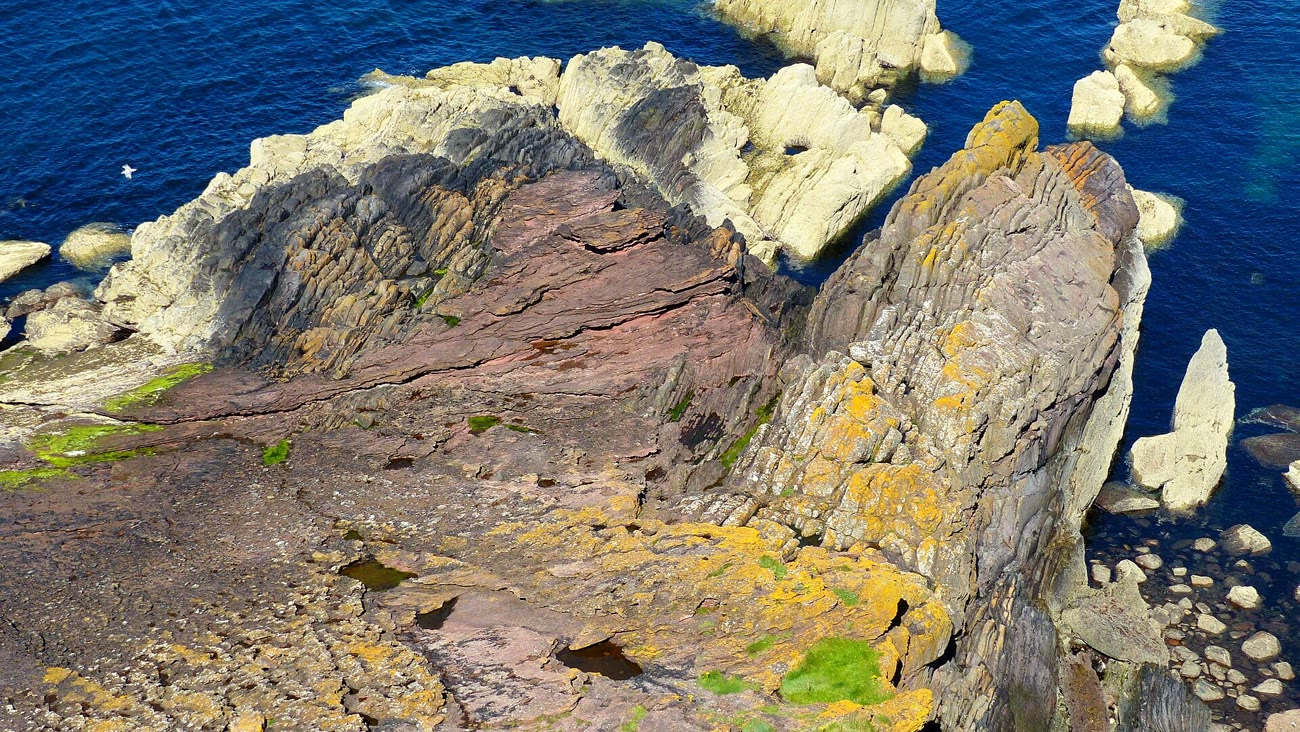
\includegraphics[width=0.7\linewidth]{images/book3/b1-siccar-point.jpg}

{\small Hutton's \omterm{def:b1:cross-sections:unconformity}{unconformity} at Siccar Point: near-vertical grey Silurian
beds below, gently inclined red Devonian beds above. Photograph Pawe\l{}S,
CC BY-SA 4.0 (Wikimedia Commons).}
% ledger: commons:siccar-point
\end{center}
\end{history}

\begin{inthefield}[Geology for a tunnel]
\begin{minipage}[t]{0.6\linewidth}\vspace{0pt}
Before a tunnel is designed, engineering geologists build sections along
its line from the \omterm{def:b1:geological-maps:geological-map}{geological map}, from boreholes drilled at intervals
along the route, and from geophysical surveys. They predict each unit the
tunnel will cut, the faults it will cross, and where water may enter. During
boring, the geologists of the contractor log the rock exposed at the face at
every advance, compare it with the prediction, and update the section;
probe holes drilled ahead of the machine test the ground before the machine
reaches it, especially near a predicted fault or in limestone that may hold
cavities. A fault zone of crushed rock is a classic hazard, all the more
when the same rock lies on both sides and nothing in the face warns of it.
\end{minipage}\hfill
\begin{minipage}[t]{0.37\linewidth}\vspace{0pt}
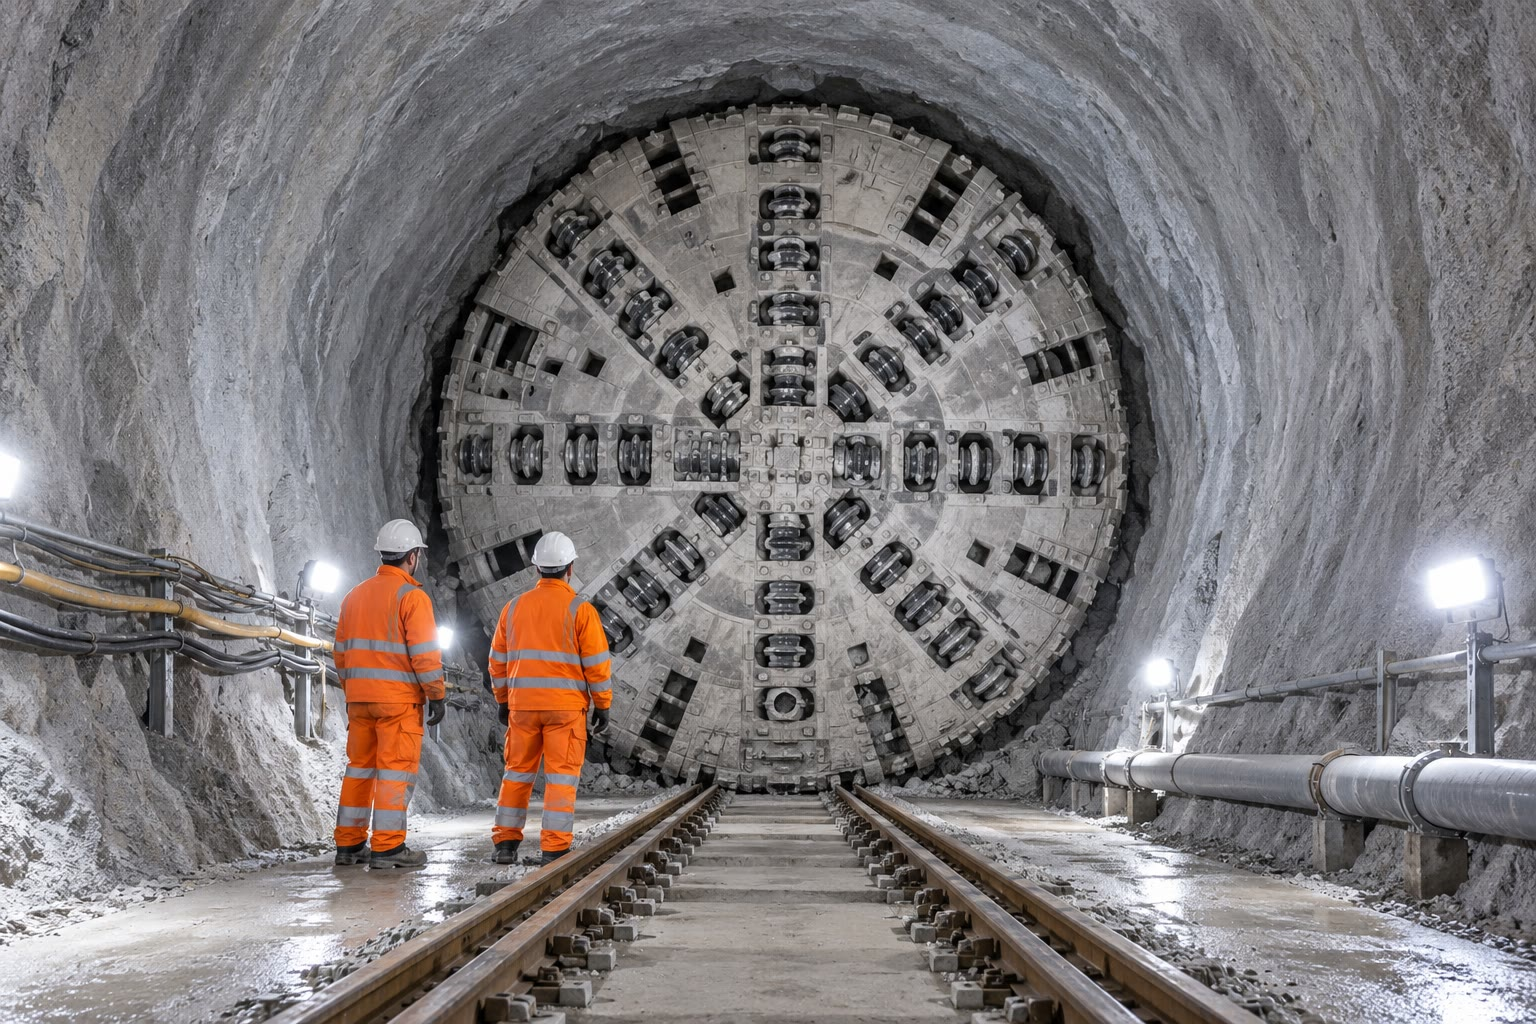
\includegraphics[width=\linewidth]{images/book3/ai/b1-tunnel-boring.jpg}
\end{minipage}
\end{inthefield}

\section{Exercises}

\begin{exercise}[$\star$]\label{exo:b1:cross-sections:1}
A section is drawn from a map at the scale 1:25\,000, with a vertical scale
of \qty{1}{cm} for \qty{100}{m}. What is its \omterm{def:b1:cross-sections:section}{vertical exaggeration}?
\end{exercise}

\begin{exercise}[$\star$]\label{exo:b1:cross-sections:2}
A bed \omterm{def:b1:geological-maps:attitude}{dips} \ang{40} toward \ang{090}. What is its \omterm{def:b1:cross-sections:apparent-dip}{apparent dip} in a vertical
section of \omterm{def:b1:spherical-astronomy:horizontal}{azimuth} \ang{060}? Of \omterm{def:b1:spherical-astronomy:horizontal}{azimuth} \ang{000}?
\end{exercise}

\begin{exercise}[$\star$]\label{exo:b1:cross-sections:3}
A vertical borehole crosses \qty{120}{m} of sandstone whose beds \omterm{def:b1:geological-maps:attitude}{dip}
\ang{12.16}. What is the \omterm{def:b1:cross-sections:thickness}{true thickness} of the sandstone?
\end{exercise}

\begin{exercise}[$\star$]\label{exo:b1:cross-sections:4}
A contact dipping \ang{12} in the plane of a section is drawn with \omterm{def:b1:cross-sections:section}{vertical
exaggerations} of 2, 3 and 5. At what angles does it appear?
\end{exercise}

\begin{exercise}[$\star\star$]\label{exo:b1:cross-sections:5}
A layer \omterm{def:b1:geological-maps:attitude}{dips} \ang{25}. Its \omterm{def:b1:geological-maps:geological-map}{outcrop} is \qty{300}{m} wide, measured
perpendicular to the \omterm{def:b1:geological-maps:attitude}{strike}. Compute its \omterm{def:b1:cross-sections:thickness}{true thickness} (a) on flat ground;
(b) on ground sloping at \ang{10} the opposite way to the \omterm{def:b1:geological-maps:attitude}{dip}, the width
being measured along the ground; (c) on ground sloping at \ang{10} the same
way as the \omterm{def:b1:geological-maps:attitude}{dip}.
\end{exercise}

\begin{exercise}[$\star\star$]\label{exo:b1:cross-sections:6}
A bed shows an \omterm{def:b1:cross-sections:apparent-dip}{apparent dip} of \ang{20} to the north in a north--south
section, and of \ang{30} to the east in an east--west section. Find its \omterm{def:b1:geological-maps:attitude}{dip
direction} and its true \omterm{def:b1:geological-maps:attitude}{dip}.
\end{exercise}

\begin{exercise}[$\star\star$]\label{exo:b1:cross-sections:7}
The base of the limestone on the east limb \omterm{def:b1:geological-maps:attitude}{dips} \ang{12.16}. What is the
horizontal spacing of its \omterm{def:b1:cross-sections:structure-contour}{structure contours} drawn every \qty{100}{m}? Check
it on the \omterm{def:b1:cross-sections:structure-contour}{structure-contour map}.
\end{exercise}

\begin{exercise}[$\star\star$]\label{exo:b1:cross-sections:8}
From the borehole table, compute the elevation of the base of the shale in
B1 and B3. Above B2 the shale has been eroded: from the \omterm{def:b1:cross-sections:thickness}{vertical thickness}
of the limestone, find the elevation its base would have there, and the
\omterm{def:b1:cross-sections:apparent-dip}{apparent dip} of that contact between B1 and B2 in section C--D. What does
the comparison of B1 and B3 tell about the \omterm{def:b1:geological-maps:fold}{fold}?
\end{exercise}

\begin{exercise}[$\star\star$]\label{exo:b1:cross-sections:9}
A normal fault dipping \ang{50} toward \ang{180} has a \omterm{def:b1:cross-sections:throw}{throw} of
\qty{150}{m}. Compute its \omterm{def:b1:cross-sections:throw}{heave}. In a vertical section of \omterm{def:b1:spherical-astronomy:horizontal}{azimuth} \ang{150},
what are the \omterm{def:b1:cross-sections:apparent-dip}{apparent dip} of the fault and the separation of the two cutoffs
of a horizontal bed along the section?
\end{exercise}

\begin{exercise}[$\star\star\star$]\label{exo:b1:cross-sections:10}
For a bed dipping \ang{40}, in which section directions is the \omterm{def:b1:cross-sections:apparent-dip}{apparent dip}
half the true \omterm{def:b1:geological-maps:attitude}{dip}, that is \ang{20}? Show that the \omterm{def:b1:cross-sections:apparent-dip}{apparent dip} varies
little near the \omterm{def:b1:geological-maps:attitude}{dip direction} and fast near the \omterm{def:b1:geological-maps:attitude}{strike}.
\end{exercise}

\begin{exercise}[$\star\star\star$]\label{exo:b1:cross-sections:11}
A borehole crosses the limestone of the east limb (\omterm{def:b1:cross-sections:thickness}{true thickness}
\qty{176.0}{m}, \omterm{def:b1:geological-maps:attitude}{dip} \ang{12.16} toward \ang{080.7}). What length of core
does it recover (a) if vertical; (b) if inclined at \ang{60} below the
horizontal toward \ang{260.7}; (c) inclined at \ang{60} toward \ang{080.7}?
(Hint: the length is $t/\cos\psi$, where $\psi$ is the angle between the
borehole and the normal to the bedding.)
\end{exercise}

\begin{exercise}[$\star\star\star$]\label{exo:b1:cross-sections:12}
At an \omterm{def:b1:cross-sections:unconformity}{angular unconformity}, the beds below \omterm{def:b1:geological-maps:attitude}{dip} \ang{70} toward \ang{090}
and the beds above \omterm{def:b1:geological-maps:attitude}{dip} \ang{20} toward \ang{270}, with the same \omterm{def:b1:geological-maps:attitude}{strike}.
Rotate the whole \omterm{def:b1:geological-maps:geological-map}{outcrop} about the \omterm{def:b1:geological-maps:attitude}{strike} to bring the upper beds back to
horizontal: what was the \omterm{def:b1:geological-maps:attitude}{dip} of the lower beds when the upper ones were
deposited? Write the history of the \omterm{def:b1:geological-maps:geological-map}{outcrop} in order.
\end{exercise}

\section{Problem: A tunnel under the Varden Hills}

\begin{problem}[{Weekend problem --- which rocks a tunnel will cut, where it
will meet the fault, and how much limestone it will bore}]
\label{pb:b1:cross-sections:1}
% numbers from figdata/bachelor-1/varden_sections.py (model region.py) and the scratch calculator
The tunnel runs due east along the line C--D ($y = \qty{6}{km}$) at the
constant elevation of \qty{200}{m}, from $x = \qty{1}{km}$ to $x =
\qty{9}{km}$. The ground elevation along C--D is, every kilometre from
$x = 0$:
\begin{center}
\small
\begin{tabular}{lccccccccccc}
\hline
$x$ (km) & 0 & 1 & 2 & 3 & 4 & 5 & 6 & 7 & 8 & 9 & 10 \\
$z$ (m) & 509 & 556 & 467 & 370 & 435 & 534 & 501 & 455 & 406 & 339 & 405 \\
\hline
\end{tabular}
\end{center}
Use the borehole table of the chapter, the section C--D drawn with $e = 3$,
the \omterm{def:b1:geological-maps:attitude}{attitude} of the east limb (\omterm{def:b1:geological-maps:attitude}{dip} \ang{12.16} toward \ang{080.7}; the west
limb is its mirror image, dipping toward \ang{279.3}), and the normal fault,
which \omterm{def:b1:geological-maps:attitude}{dips} \ang{60} toward \ang{120}, has a \omterm{def:b1:cross-sections:throw}{throw} of \qty{200}{m}, and
passes through the point $x = \qty{4.30}{km}$, $y = \qty{1.00}{km}$,
$z = \qty{250}{m}$.

\medskip
\noindent\textbf{Part I --- The profile and the units.}
\begin{enumerate}
  \item What are the greatest and the smallest thicknesses of rock above the
        tunnel at the kilometre points between $x = 1$ and $x = 9$?
  \item On the printed section, \qty{1}{km} of horizontal distance measures
        \qty{1.4}{cm} and \qty{1}{km} of elevation measures \qty{4.2}{cm}.
        Check that $e = 3$.
  \item From log B2, find the elevation of the base of the sandstone on the
        crest of the \omterm{def:b1:geological-maps:fold}{anticline}.
  \item In which unit is the tunnel at $x = \qty{3.5}{km}$?
  \item Compute the elevation of the base of the limestone in B1 and B3.
  \item From the section, list in order the units the tunnel crosses from
        $x = 1$ to $x = \qty{9}{km}$.
\end{enumerate}

\medskip
\noindent\textbf{Part II --- Dips in the section.}
\begin{enumerate}[resume]
  \item Compute the \omterm{def:b1:cross-sections:apparent-dip}{apparent dip} of the east limb in C--D from its \omterm{def:b1:geological-maps:attitude}{attitude}.
  \item Check it from the elevations of the base of the limestone in B2 and
        B3.
  \item At what angle is the east limb drawn in the section with $e = 3$?
  \item Compute the \omterm{def:b1:cross-sections:apparent-dip}{apparent dip} of the fault in C--D.
  \item Why is the \omterm{def:b1:cross-sections:apparent-dip}{apparent dip} of the limbs in C--D so close to their true
        \omterm{def:b1:geological-maps:attitude}{dip}, and that of the fault less so?
\end{enumerate}

\medskip
\noindent\textbf{Part III --- The fault.}
\begin{enumerate}[resume]
  \item Show that, on the plane $y = \qty{6}{km}$, the fault lies at
        \[ x = 4300 + \frac{2500 - (z - 250)\tan\ang{30}}{\sin\ang{120}}
           \quad\text{(metres)}. \]
  \item Where does the tunnel meet the fault?
  \item Compute the \omterm{def:b1:cross-sections:throw}{heave} of the fault, and the separation of the cutoffs of
        a contact along C--D.
  \item Which block is downthrown, and which unit lies at tunnel level on each
        side of the fault?
  \item Why is the fault a hazard that the tunnelling crew could not see
        coming from the rock at the face? How do the engineers guard against
        it?
\end{enumerate}

\medskip
\noindent\textbf{Part IV --- The limestone.}
\begin{enumerate}[resume]
  \item What is the \omterm{def:b1:cross-sections:thickness}{vertical thickness} of the limestone in B1?
  \item What is its \omterm{def:b1:cross-sections:thickness}{true thickness}?
  \item Show that, west of the fault on C--D, the base of the sandstone lies
        at
        \[ z_b = 160.16 - |x - 3500|\tan\ang{12.0} \quad\text{(metres)}. \]
  \item The tunnel is in the limestone when its base lies below \qty{200}{m}
        and its top above. Show that this happens for $377.1 < |x - 3500|
        < 1224.0$.
  \item Give the four points where the tunnel enters and leaves the
        limestone.
  \item Show that the length bored on each limb is $h/\tan\beta$, where $h$
        is the \omterm{def:b1:cross-sections:thickness}{vertical thickness} and $\beta$ the \omterm{def:b1:cross-sections:apparent-dip}{apparent dip}, and compute
        it.
  \item What total length of limestone does the tunnel bore through?
\end{enumerate}
\end{problem}
